\subsection{Công nghệ lưu trữ - Redis}
Redis~\cite{redis:online} là viết tắt của Remote Dictionary Server
(máy chủ từ điển từ xa), lưu trữ dữ liệu dưới dạng
KEY-VALUE trong bộ nhớ. Là phần mềm mã nguồn mở có tốc độ
truy cập nhanh để dùng làm cơ sở dữ liệu đơn giản, bộ nhớ đệm (cache),
trình chuyển tiếp (broker) tin nhắn hoặc
được sử dụng làm danh sách tác vụ chờ xử lý (queue). 

Redis hiện cung cấp thời gian phản hồi ở tốc độ chưa đến
một mili giây, giúp thực hiện hàng triệu yêu cầu mỗi giây cho
các ứng dụng thời gian thực trong lĩnh vực Trò chơi, Quảng cáo, Dịch
vụ tài chính, Chăm sóc sức khoe, IoT, … Cụ thể, Redis thường được chọn
sử dụng cho các hoạt động lưu trữ bộ nhớ đệm, quản lý phiên, trò chơi,
bảng xếp hạng, phân tích thời gian thực, dữ liệu không gian
địa lý, ứng dụng đặt xe, trò chuyện / nhắn tin, phát trực tiếp
nội dung đa phương tiện, …

Redis là một cơ sở dữ liệu NoSQL. NoSQL là một dạng cơ sở dữ liệu
phi quan hệ, sử dụng nhiều loại mô hình dữ liệu đa dạng để
truy cập và quản lý dữ liệu trong bộ nhớ và tìm kiếm, NoSQL được
tối ưu hóa dành riêng cho các ứng dụng yêu cầu mô hình dữ liệu
linh hoạt có lượng dữ liệu lớn và độ trễ thấp, đạt được bằng cách
giảm bớt một số hạn chế về tính nhất quán của dữ liệu.

\begin{figure}[H]
    \centering
    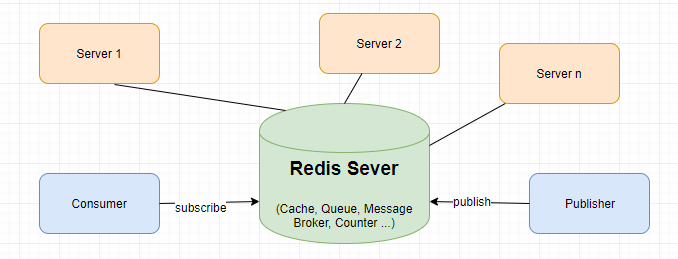
\includegraphics[width=14cm]{images/redis.png}
    \caption{Redis server}
\end{figure}

\textit{Cách thức hoạt động của Redis:}

Toàn bộ dữ liệu của Redis nằm trong bộ nhớ (RAM), khác với những loại 
cơ sở dữ liệu thông thường khác lưu dữ liệu trên ổ đĩa hoặc ổ SSD. 
Phần lớn các tác vụ trên cơ sở dữ liệu truyền thống đều yêu cầu 
truy cập qua lại tới ổ đĩa, do vậy sẽ tốn thời gian tìm kiếm, 
dữ liệu của Redis nằm trên RAM nên sẽ không mất thời gian này. 
Do đó Redis có thể hỗ trợ thêm khá nhiều tác vụ và có thời gian 
phản hồi nhanh hơn. Hiệu suất của Redis rất tốt với các tác 
vụ đọc ghi thông thường mất chưa đầy một mili giây và hỗ trợ 
hàng triệu tác vụ mỗi giây. 

Khác với các cơ sở dữ liệu quan hệ như MySQL hay PostgreSQL,
Redis không có bảng. Redis lưu dữ liệu dưới dạng KEY-VALUE và hỗ
trợ nhiều cấu trúc dữ liệu cơ bản như hash, list, set,
sorted set, string, … Bên cạnh đó Redis có 2 background threads chuyên
làm nhiệm vụ định kì ghi dữ liệu trên đĩa cứng, cơ chế backup
này giúp cho Redis có độ bảo mật và sửa lỗi cao.

\textit{Một số ứng dụng phổ biến của Redis:}
\begin{itemize}[topsep=0ex]
\item Lưu trữ bộ nhớ đệm (caching): Sử dụng bộ nhớ đệm để giảm độ trễ
    khi truy cập dữ liệu, tăng năng suất và giảm tải cho cơ sở dữ
    liệu và ứng dụng của bạn. Redis có thể phục vụ những dữ liệu thường
    xuyên được yêu cầu với thời gian phản hồi chưa đến một mili giây
    và cho phép dễ dàng thay đổi quy mô nhằm đáp ứng mức tải cao hơn
    mà không cần tốn kém chi phí vào back-end.

\item Bảng xếp hạng game: Redis là giải pháp hay được các nhà phát
    triển game dùng để xây dựng bảng xếp hạng theo thời gian thực
    (real-time leaderboard). Sử dụng cấu trúc dữ liệu Sorted Set của
    Redis, cấu trúc dữ liệu này đảm bảo tính duy nhất của các thành
    phần trong khi vẫn duy trì danh sách được sắp xếp theo điểm số
    của người dùng. Danh sách cập nhật mỗi khi điểm số người dùng thay đổi.

\begin{figure}[H]
    \centering
    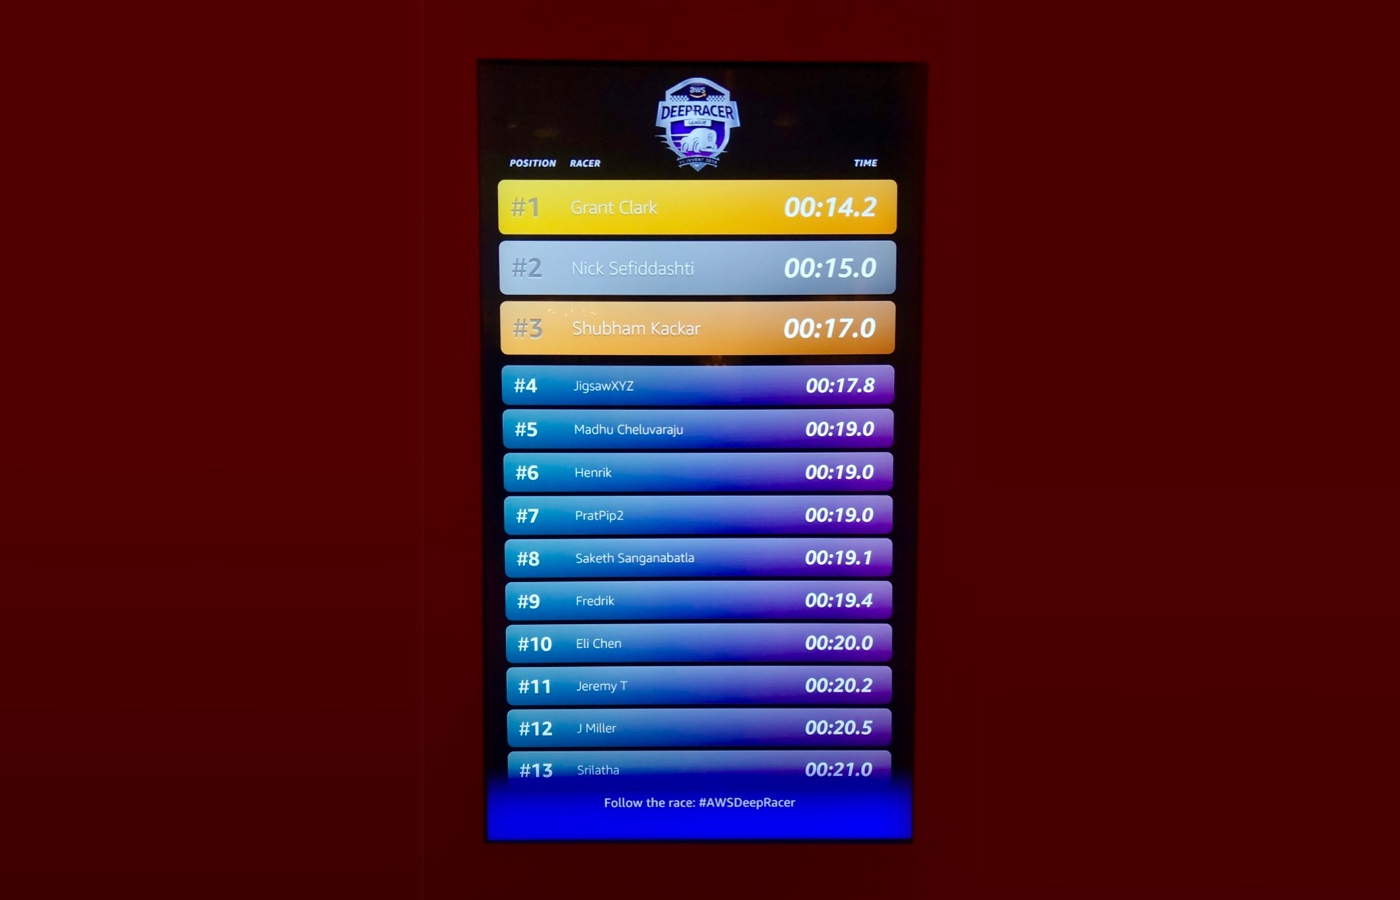
\includegraphics[width=10cm]{images/real-time-leaderboard.jpg}
    \caption{Ứng dụng Redis trong bảng xếp hạng game}
\end{figure}

\item Lưu trữ phiên (session): Các nhà phát triển ứng dụng thường sử
    dụng Redis để lưu trữ, quản lý phiên cho các ứng dụng quy mô
    Internet. Quản lý dữ liệu phiên chẳng hạn như hồ sơ người dùng,
    thông tin xác thực đăng nhập (token), trạng thái phiên, …

\item Trò chuyện, nhắn tin, hàng chờ xử lý tác vụ: Redis hỗ trợ Pub/Sub
    (là cấu trúc gửi – nhận tin nhắn mà người gửi và người nhận không
    biết nhau) với nhiều cấu trúc dữ liệu như list, sorted set, hash.
    Điều này cho phép Redis hỗ trợ những chat rooms hiệu năng cao,
    luồng tin nhắn theo thời gian thực.
\end{itemize}

\textit{So sánh Redis và một loại cơ sở dữ liệu quan hệ thông thường (MySQL)}
\begin{table}[H]
\centering
\begin{tabular}{| m{3cm} | m{6cm} | m{6cm} |}
\hline
& \textbf{Redis} & \textbf{MySQL} \\ 

\hline
\multirow{5}{3cm}{Cấu trúc cơ sở dữ liệu} &
Lưu trữ dạng KEY-VALUE & Lưu trữ dạng bảng \\  
\cline{2-3}
& Lưu dữ liệu trong RAM, là máy chủ cấu trúc dữ
liệu vì các key có thể chứa string, hash, list,
set và sorted set
& MySQL cung cấp một máy chủ cơ sở dữ liệu quan hệ SQL
rất nhanh, đa luồng, đa người dùng, mạnh mẽ \\  

\hline
\multirow{9}{3cm}{Ưu điểm}
& $\bullet$ Dễ cài đặt, sử dụng, deploy, maintain, … & 
$\bullet$ Cơ sở dữ liệu quan hệ mã nguồn mở được sử dụng rộng rãi \\
& $\bullet$ Lưu trữ dữ liệu trong bộ nhớ nên cho hiệu
    năng cao và tốc độ nhanh &
$\bullet$ Dễ sử dụng, khả năng tương thích cao, hỗ trợ đa nền tảng,
cộng đồng phát triển mạnh mẽ \\
& $\bullet$ Mã nguồn mở, ổn định, chi phí hiệu quả &
$\bullet$ Hỗ trợ index và full-text searching \\
& $\bullet$ Khả năng mở rộng cao, hỗ trợ sao lưu vào đĩa cứng & \\
& $\bullet$ Cấu trúc dữ liệu đa dạng & \\
\hline
\multirow{5}{3cm}{Trường hợp nên sử dụng} & 
$\bullet$ Có dữ liệu dạng KEY-VALUE & $\bullet$ Cần cơ sở dữ liệu quan hệ \\
& $\bullet$ Cần lưu cache & $\bullet$ Khi có các hoạt động phân tán \\
& $\bullet$ Cần hiệu năng cao &
$\bullet$ Cần bảo mật cao và hoạt động đơn giản \\
& $\bullet$ Kích thước dữ liệu ổn định &
$\bullet$ Không sử dụng khi dữ liệu lớn dần và 
không thể cache hết lên bộ nhớ \\
\hline
\multirow{3}{3cm}{Nhược điểm} & 
$\bullet$ Redis sử dụng RAM nên khi lượng file cache lớn sẽ
dẫn đến thiếu RAM cho server &
$\bullet$ Nhiều vấn đề về lưu trữ procedure và trigger \\
& $\bullet$ Không thể truy vấn trực tiếp các object & \\
\hline
\end{tabular}
\caption{So sánh Redis và MySQL}
\end{table}
